\subsection{Validation de l'étatpe 1}

Les simulations effectuées ont permis d'obtenir les résultats suivants, qui montrent que le modèle de contrôle appliqué donne des résultats satisfaisants. 
 
 Analisant les résultats du modèle Simulink de la figure \ref{img:simulink1}, on a que le robot s'oriente initialement vers $-\pi$, puis effectue un demi-tour pour atteindre l'origine. Toutefois, il perd du temps en effectuant un tour supplémentaire sur lui-même avant d'atteindre sa destination.

\begin{figure}[!h]
    \centering
    \includegraphics[width=1.0\textwidth]{img/diagrams/5courbe_trajectoire.png} 
    \caption{Résultat de la simulation pour $x_0 = -2$, $y_0 = -4$, $\theta_0 = -\pi$}
    \label{img-abc_dq}
\end{figure}
\FloatBarrier

Résultats de la simulation du modèle Simulink de la figure \ref{img:simulink2} : Ici on observe que le robot effectue un trajet plutôt logique et peut être saccadé.

\begin{figure}[!h]
    \centering
    \includegraphics[width=1.0\textwidth]{img/diagrams/7.png} 
    \caption{Résultat de la simulation pour $x_a = 10$, $y_a = -3$, $\theta_a = -pi/4$ pour A et $\x^* = 4$, $\y^* = -1$, $\theta^* = 0$ pour B}
    \label{img-abc_dq}
\end{figure}

\FloatBarrier

\subsection{Validation de l'étape 2}

Dans cette étape, la validation du suivi de trajectoire du robot à l'aide de l'algorithme de recherche A* (\textit{star search}) a d'abord été effectuée. Un cycle a été créé qui marquait des points aléatoires sur la carte, et il a été possible de voir l'efficacité du code pour trouver des points proches des points marqués sur la trajectoire et pour trouver le chemin minimal entre eux, comme le montre l'image \ref{img:trajectory} qui enregistre le test.

\begin{figure}[!h]
    \centering
    \includegraphics[width=0.6\textwidth]{img/background/trajectory.png} 
    \caption{Validation de l'algorithme de recherche en étoile en trouvant la trajectoire minimale entre deux points passant par les rues.}
    \label{img:trajectory}
\end{figure}

\FloatBarrier

Après avoir validé l'algorithme, le développement du nœud de contrôle automatique a été possible, où l'utilisateur cliquerait sur deux points et le robot suivrait sa trajectoire. Dans l'interface, deux modes ont été créés : un pour une trajectoire en ligne droite reliant les points et un autre pour une trajectoire suivant les rues, qui serait calculée par l'algorithme de recherche A*. 

L'implémentation de l'algorithme dans l'interface a été réalisée, générant même une animation du véhicule se déplaçant sur la carte. Cependant, dans le mode suivant la trajectoire de la rue, le code a présenté quelques bugs. Nous avons conclu que ces bugs provenaient d'une erreur de codage, confondant les coordonnées utilisées par l'algorithme de recherche A* et celles utilisées par l'interface Tkinter. Pour expliquer brièvement, l'algorithme A* utilise des coordonnées basées sur la grille de la carte, tandis que Tkinter utilise des coordonnées de l'écran, nécessitant une conversion entre ces deux systèmes.

De plus, malheureusement, il n'a pas été possible d'implémenter le contrôle de ces algorithmes par la publication en temps réel sur les topics de vitesse linéaire et d'angle des roues comme prévu. Les résultats des simulations de l'interface en fonctionnement dans les modes de parcours du chemin en ligne droite et via les rues peuvent être vus dans les images \ref{img:linear_line} et \ref{img:street_line}.

\FloatBarrier
\begin{figure}[!h]
    \centering
    \includegraphics[width=0.6\textwidth]{img/background/linear_line.png} 
    \caption{Simulation de l'application de la trajectoire en mode trajectoire linéaire.}
    \label{img:linear_line}
\end{figure}

\FloatBarrier

\begin{figure}[!h]
    \centering
    \includegraphics[width=0.6\textwidth]{img/background/street_line.png} 
    \caption{Simulation de l'application de la trajectoire en mode trajectoire suivant la trajectoire des rues.}
    \label{img:street_line}
\end{figure}
\FloatBarrier


\subsection{Tests avec le robot Agilex Limo}

Après avoir testé les méthodes de contrôle et codé les nœuds et algorithmes en Python, il a été possible de réaliser des tests sur le robot modèle Limo. Pour accéder au robot, ses ports USB latéraux ont été utilisés pour la connexion de clés USB pour le transfert de fichiers, ainsi que pour la connexion de périphériques tels qu'une souris et clavier. Le robot fonctionne avec un ordinateur intégrant un système d'exploitation Linux, accessible via son écran tactile. Pour faciliter l'accès et le travail avec le robot, le logiciel NoMachine \cite{NoMachine} a également été utilisé. Les tests ont été réalisés dans le laboratoire H4 de l'ENSEM ou dans les salles informatiques de l'institution. Les photos \ref{img:code} et \ref{img:acess} montrent comment les connexions au robot étaient effectuées pour travailler avec lui, exécuter les codes, etc.

\begin{figure}[!h]
    \centering
    \includegraphics[width=0.6\textwidth]{img/agilex/code.jpg} 
    \caption{Manipulation du robot à partir du logiciel NoMachine.}
    \label{img:code}
\end{figure}
\FloatBarrier


\begin{figure}[!h]
    \centering
    \includegraphics[width=0.6\textwidth]{img/agilex/acess.jpg} 
    \caption{Accès à l'interface du robot via les ports USB.}
    \label{img:acess}
\end{figure}
\FloatBarrier

Pour permettre l'exécution des codes sur le robot, l'installation de diverses bibliothèques et paquets non préinstallés était nécessaire, ainsi que la modification de fichiers de configuration et la suppression de modules tels que ROS1, préinstallé mais entrant en conflit avec le ROS2 utilisé dans le projet.

Pour les tests, le robot a été positionné soit dans l'environnement de test, soit sur sa base, pour pouvoir exécuter les commandes sans se déplacer, comme le montrent les images \ref{img:track1} et \ref{img:base} respectivement.

\begin{figure}[!h]
    \centering
    \includegraphics[width=0.6\textwidth]{img/agilex/1track.jpg} 
    \caption{Robot testé sur la piste d'essai du laboratoire H4 de l'ENSEM.}
    \label{img:track1}
\end{figure}
\FloatBarrier

\begin{figure}[!h]
    \centering
    \includegraphics[width=0.6\textwidth]{img/agilex/base.jpg} 
    \caption{Robot exécutant des commandes positionné sur une base.}
    \label{img:base}
\end{figure}
\FloatBarrier

L'environnement a également été mesuré à l'aide d'une règle disponible dans le laboratoire pour référence, comme le montre l'image \ref{img:track2}.

\begin{figure}[!h]
    \centering
    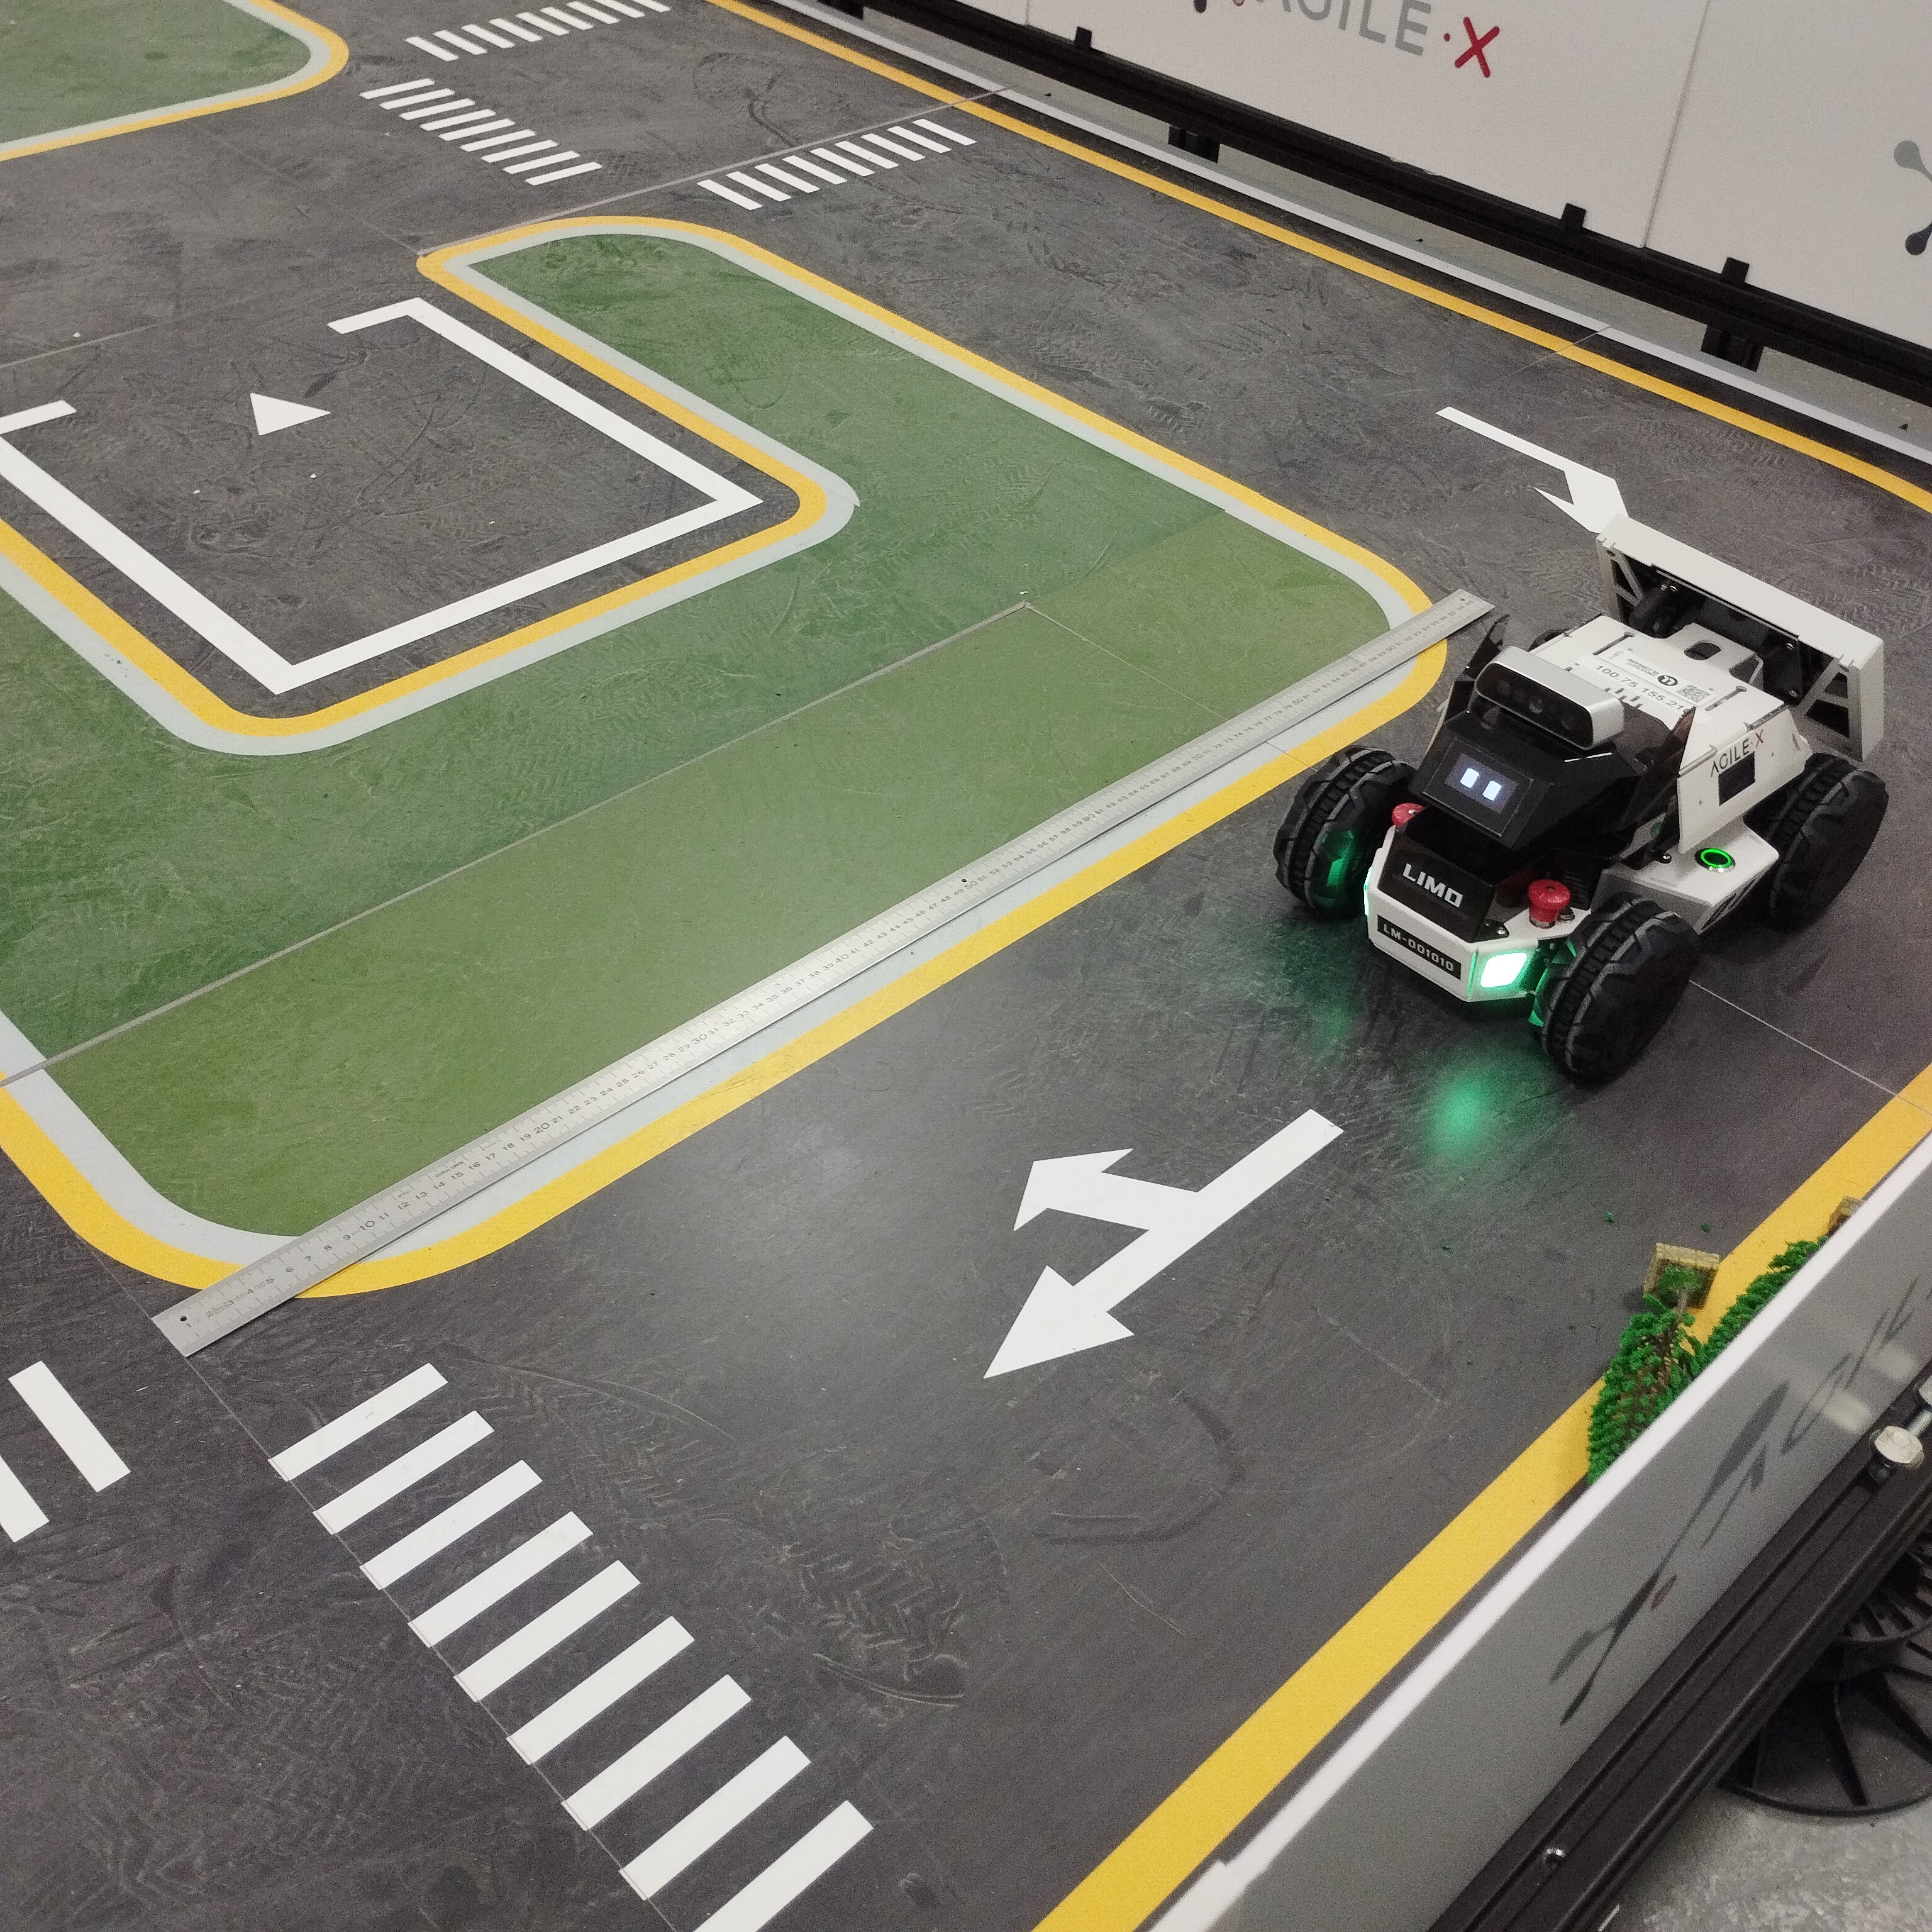
\includegraphics[width=0.6\textwidth]{img/agilex/2trackup.jpg} 
    \caption{Référence des proportions, du robot et de l'environnement proche d'une règle d'un mètre. }
    \label{img:track2}
\end{figure}
\FloatBarrier

Il a été possible de réaliser des tests de mouvement du robot via l'application de commandes ROS en utilisant l'interface Tkinter développée à cet effet, comme le montre l'image \ref{img:click}.

\begin{figure}[!h]
    \centering
    \includegraphics[width=0.6\textwidth]{img/agilex/click.png} 
    \caption{Interface de contrôle générée à l'aide de la bibliothèque TKinter.}
    \label{img:click}
\end{figure}
\FloatBarrier

Certains modules natifs de ROS, tels que \textit{turtlesim} et \textit{rqtgraph}, ont également facilité le travail de simulation, permettant de visualiser l'exécution des nœuds et des topics et leur communication mutuelle. Ceci peut être observé à travers l'image \ref{img:rqt_graph}.

\begin{figure}[!h]
    \centering
    \includegraphics[width=0.6\textwidth]{img/agilex/rqt_graph.png} 
    \caption{Graphique ROS de la bibliothèque RQT.}
    \label{img:rqt_graph}
\end{figure}
\FloatBarrier

Ainsi, la seule chose qui restait était le fonctionnement du nœud d'application de commande de trajectoires automatiques. Dans ce nœud, il n'a pas été possible d'implémenter la partie qui publie les commandes au robot en temps réel. De plus, les nœuds de caméra ou de lidar natifs du robot auraient pu être utilisés pour une meilleure identification des éléments sur la piste, améliorant le contrôle ou réalisant d'autres fonctions. D'autres améliorations possibles seraient l'implémentation de la publication des informations des nœuds sur les réseaux pour un accès à distance, permettant ainsi d'utiliser les connaissances acquises à l'ENSEM dans les disciplines de l'IOT pour exécuter certains nœuds sur une machine et récupérer les informations publiées par ces nœuds sur le robot via l'accès à un serveur ou quelque chose de similaire. Plusieurs applications n'ont pas été explorées, comme l'utilisation d'une commande sans fil pour le contrôle manuel, entre autres.

